\chapter{本手法を用いた初段ミューオントリガーの性能評価}
実際にRun-3での性能について書く
位置依存性とか大量に

\subsection{作成した CW の評価}
Run-2データを用いた評価

<15段階の閾値のEfficiency>
\begin{figure}[tb]
  \centering
  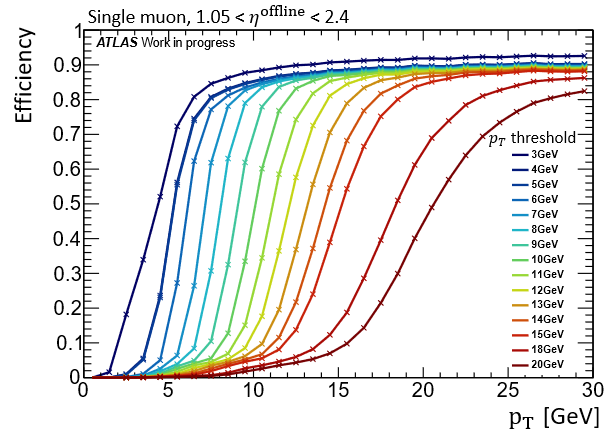
\includegraphics[clip, width=14cm]{fig/4/v07_15_Eff.png}
  \caption{Resolution}
  \label{fig:Resolution}
\end{figure}


<15段階それぞれのEfficiency(v05 vs v06,v07)>\\
\begin{figure}[tb]
  \centering
  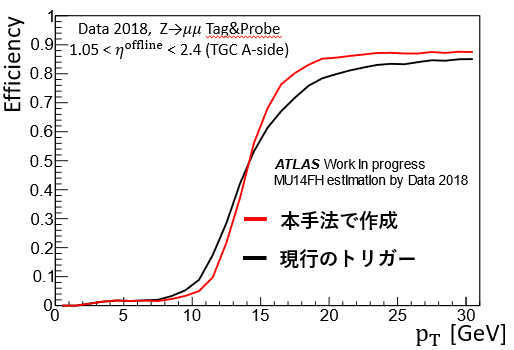
\includegraphics[clip, width=14cm]{fig/4/hikaku_v05_v06.png}
  \caption{v05v06}
  \label{fig:Resolution}
\end{figure}

\begin{figure}[tb]
  \centering
  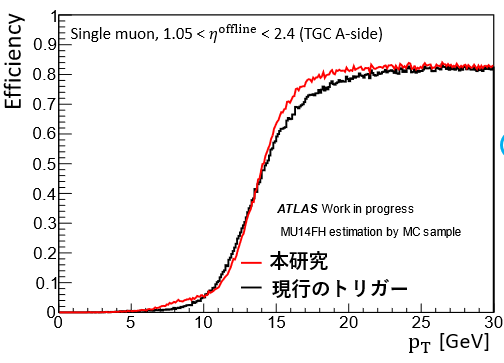
\includegraphics[clip, width=14cm]{fig/4/hikaku_v05_v07.png}
  \caption{v05v07}
  \label{fig:Resolution}
\end{figure}

<MCとDataの比較>
\begin{figure}[tb]
  \centering
  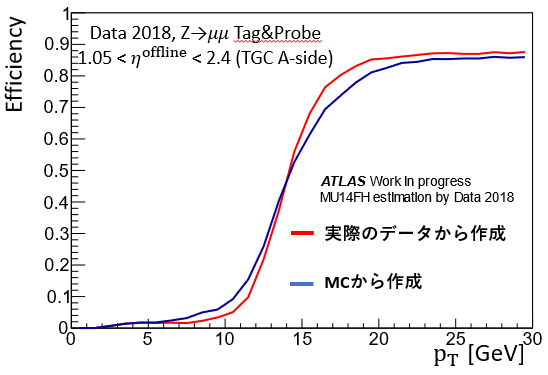
\includegraphics[clip, width=14cm]{fig/4/hikaku_v06_v07.png}
  \caption{v06v07}
  \label{fig:Resolution}
\end{figure}

<TriggerRate>
\begin{figure}[tb]
  \centering
  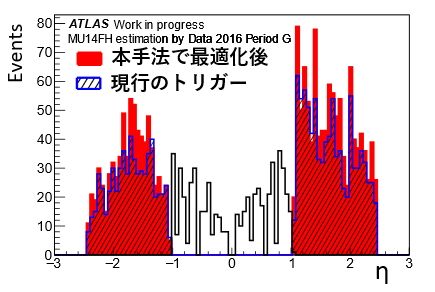
\includegraphics[clip, width=14cm]{fig/4/rate_v05_v06.png}
  \caption{v05v06}
  \label{fig:Resolution}
\end{figure}





\section{機械学習を用いることによる CW 作成の効果}
\subsubsection{チェンバーごとのEfficiency}
\begin{figure}[tb]
  \centering
  \rule{8cm}{6cm}
  %\includegraphics[clip, width=14cm]{}
  \caption{チェンバーごとのEfficiency (1-48)}
  \label{fig:fit_def}
\end{figure}

\subsubsection{ミューオンの電荷に対する効果}

\begin{figure}[tb]
  \centering
  \rule{8cm}{6cm}
  %\includegraphics[clip, width=14cm]{}
  \caption{Rate}
  \label{fig:fit_def}
\end{figure}


\section{Run-3に向けた本手法のトリガー性能}
Date と MC でeffの比較
\begin{figure}[tb]
  \centering
  \rule{8cm}{6cm}
  \caption{Efficiency}
  \label{fig:fit_def}
\end{figure}

\subsection{トリガーレート}
Date と MC
\begin{figure}[tb]
  \centering
  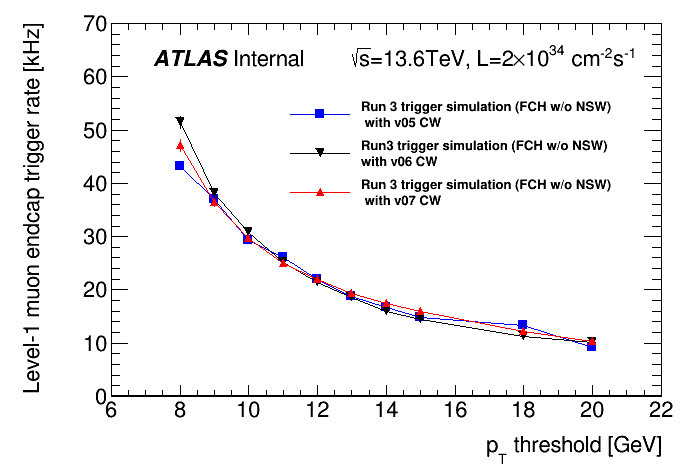
\includegraphics[clip, width=14cm]{fig/5/l1mue_rate_run3.png}
  \caption{Rate}
  \label{fig:fit_def}
\end{figure}

